\documentclass{subfiles}
\begin{document}
Altro aspetto legato all'analisi di immagini è il contrasto: si intenda questi come l'accentazione dei dettagli di un immagine.
L'aumento di contrasto in un immagine digitale è effettuato tramite i filtri di sharpening.
L'idea alla base è molto semplice: proprio perché ciò a cui si è interessati è
\begin{wrapfigure}[13]{r}{0.425\textwidth}
    \centering
    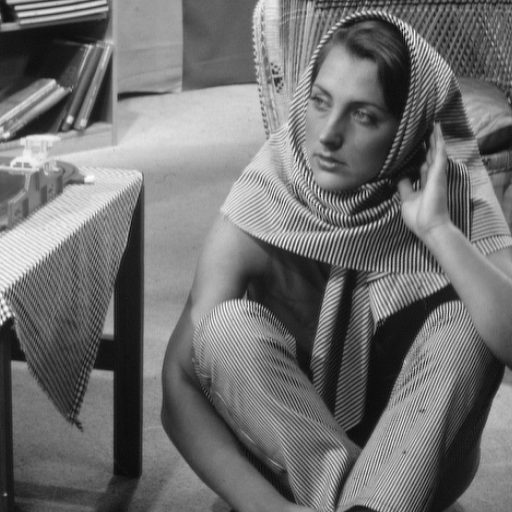
\includegraphics[scale = 0.325]{../Images/Barbara/BarbaraGS.png}
    \caption{BarbaraGS.}
    \label{fig:4.6}
\end{wrapfigure}
esaltare i dettagli, se ad un immagine \(I\) si sottrae una sua convoluzione,
eventualmente ottenuta con un filtro di media, quel che si ottiene è un'immagine \(D\) contenente i dettagli di \(I\). Dunque se ad \(I\) si somma \(D\),
quest'ultima moltiplicata eventualmente per un qualche \(k\), quel che si ottiene è appunto l'immagine contrastata.

Per comprende l'applicazione dei filtri di sharpening, si consideri \emph{Figura \ref{fig:4.6}}.
Applicando ad essa il seguente codice MATLAB, che effettua lo sharpening secondo quanto descritto, quel che si ottiene è mostrato in \emph{Figura \ref{fig:4.7}}.
\begin{center}
    \begin{lstlisting}[language = MATLAB]
        % caricamento di BarbaraGS.png
        ker = fspecial('average', [5, 5]);
        meanB = uint8(conv2(BarbaraGS), ker, `same');
        sharp = BarbaraGS + 2.5*(BarbaraGS - meanB);
        figure; imshow(sharp, [0, 255]);
    \end{lstlisting}
\end{center}

Analizzando il codice utilizzato, la funzione \lstinline[language = MATLAB]{fspecial('average', [5, 5])} è equivalente all'istruzione
\lstinline[language = MATLAB]{ones(5)/25}, cioè essa un kernel 5 x 5 i cui valori sono normalizzati.
La restante parte del codice
\begin{wrapfigure}{l}{0.425\textwidth}
    \centering
    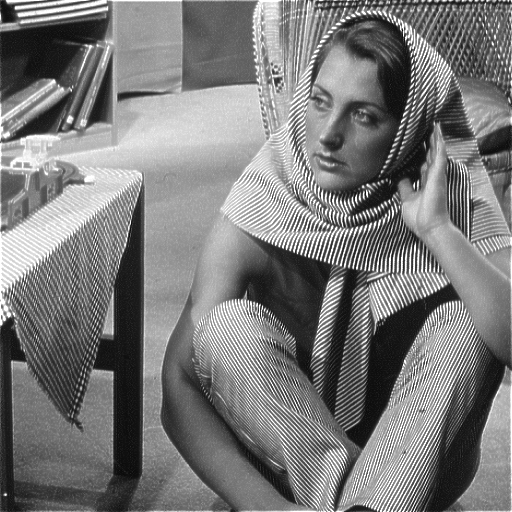
\includegraphics[scale = 0.325]{../Images/Barbara/SharpBarbara.png}
    \caption{\emph{Figura \ref{fig:4.6}} sottoposta a filtro di sharpening.}
    \label{fig:4.7}
\end{wrapfigure}
opera secondo la logica precedentemente descritta.

\begin{Note*}
    nel codice utilizzato il valore di \(k\) è posto a 2.5 unicamente per permettere di apprezzare l'effettiva applicazione del filtro,
    in generale valori elevati sono sconsigliati.
\end{Note*}

Volendo utilizzare una versione del codice meno verbosa, quindi piu sintetica e leggibile, il codice precedentemente descritto può essere sostituito con quello a seguire.
\begin{center}
    \begin{lstlisting}[language = MATLAB]
        % caricamento di BarbaraGS.png
        sharp = imsharpen(BarbaraGS);
        figure; imshow(sharp, [0, 255]);
    \end{lstlisting}
\end{center}

\begin{Remark*}
    si tenga a mente che i due codici sono del tutto equivalenti, nessuna delle due implementazioni è superiore all'altra.
\end{Remark*}
\end{document}